\documentclass[11pt]{beamer}
\usetheme{Warsaw}
\usepackage[utf8]{inputenc}
\usepackage{natbib}
\usepackage{amsmath}
\usepackage{graphicx}
\usepackage{subcaption}
\usepackage{tikz}
\usepackage{hyperref}
\setbeamertemplate{footline}[frame number]

\hypersetup{
    colorlinks=true,
    linkcolor=white,
    filecolor=magenta,      
    urlcolor=blue,
}


\title{UE COM}
\subtitle{Learning Deep CNN Denoiser Prior for Image Restoration}
\author{Adrien Zabban}
\date{8 janvier 2024}

\begin{document}

\maketitle

% \section{Introduction}
\begin{frame}{Le problème inverse}
    \begin{block}{But}
        On a une image observée dégradée $y$ et l'on veut retrouver l'image d'origine $x$. On sait 
        que cette image a été dégradée de la façon suivante : 
        $$y = Hx + v$$
        où $H$ est la matrice de 
        dégradation que l'on connait, et $v$ est un bruit gaussien d'écart-type $\sigma$ inconnu.
    \end{block}
    \begin{figure}[b]
        \centering
        
\includegraphics[width=0.25\textwidth]{../images/hqs_original/0823.png}
        \begin{tikzpicture}[overlay, remember picture]
            \draw[->, blue, very thick] (0,1.5) -- (1,1.5) node[midway, above, blue] {$f_{H, \sigma}$};
        \end{tikzpicture}
        \hspace{1cm}
        
\includegraphics[width=0.25\textwidth]{../images/hqs_constant/y.png}
        \caption{image d'origine x (à gauche) et l'image dégradée y (à droite).}
    \end{figure}
\end{frame}


\begin{frame}{Maximiser la log-likelihood}
    \begin{visibleenv}<1->
        \begin{align*}
            \text{arg} \max_x \log(p(x|y)) &= \text{arg} \max_x \log(p(x, y)) \quad \text{car } p(x|y) = \frac{p(x, y)}{p(y)} \\
            &= \text{arg} \max_x \log(p(y|x)) + \log(p(x)) \\
            &\quad \text{or } (y|x) = (v+Hx|x) \sim \mathcal{N}(Hx, \sigma^2) \\
            &= \text{arg} \max_x -\frac{\lVert y-Hx \rVert ^2}{2 \sigma^2} + \log(p(x)) \\
            &= \text{arg} \min_x \frac{1}{2}\lVert y-Hx \rVert ^2 + \lambda \Phi(x) \quad \text{avec } \Phi = -\frac{\log \circ p}{\lambda}
        \end{align*}
    \end{visibleenv}

    \begin{visibleenv}<2->
        \begin{alertblock}{But}
            On veut donc trouver $\hat{x}$ tel que : $\hat{x} = \text{arg} \displaystyle \min_x \frac{1}{2} \lVert y-Hx \rVert ^2 + \lambda \Phi(x)$
        \end{alertblock}
    \end{visibleenv}
\end{frame}

% \section{Les méthodes d'optimisation}
\begin{frame}{Une première méthode : ISTA}
    On veut minimiser : $F = f + g$ avec $f$ dérivable et $g$ pas forcément continue.
    % avec $f(x)=\frac{1}{2}\lVert y - Hx \rVert ^2$ et $g(x)=\lambda \Phi(x)$
    On pose $L$ la constante de Lipschitz de $f$.

    En posant $p_L$ tel que : $$ p_L(y) = \arg \max_x \Bigg\{ g(x) + \frac{L}{2} \Big\lVert x - \Big(y - \frac{1}{L} \nabla f(y)\Big) \Big\rVert ^2 \Bigg\}$$

    On peut montrer qu'il est possible d'approximer $\hat{x} = \displaystyle \min_x F(x)$ en itérant :
    $$x_{k+1} = p_L(x_k)$$
    c'est-à-dire : $\hat{x} = \displaystyle \lim_{k \rightarrow \infty} x_{k+1}$

\end{frame}

\begin{frame}{Une première méthode : ISTA}
    image de l'implémentation d'ISTA (si j'ai le temps) (diapo pas encore faite)
\end{frame}

\begin{frame}{Une deuxième méthode : Half Quadratic Splitting (HQS)}
    \begin{visibleenv}<1->
        \begin{exampleblock}{Idée}
            Diviser la variable $x$ pour découpler le terme de fidélité et le terme de régularisation.
        \end{exampleblock}
    \end{visibleenv}
    \begin{visibleenv}<2->
        On a l'équivalence entre :
        $$ \min_x \frac{1}{2}\lVert y-Hx \rVert^2 + \lambda \Phi(x) $$
        $$ \Leftrightarrow \min_{x, z} \frac{1}{2}\lVert y-Hx \rVert ^2 + \lambda \Phi(z) \quad \text{tel que} \quad  z=x$$
        En rajoutant un paramètre $\mu$:
        $$ \Leftrightarrow \min_{x, z}  \frac{1}{2}\lVert y-Hx \rVert ^2+\lambda \Phi(z) + \frac{\mu}{2}\lVert z-x \rVert ^2 $$
        On appelle $\mathcal{L}_{\mu}(x,z)$, le terme que l'on doit minimiser.
    \end{visibleenv}
\end{frame}

\begin{frame}{Une deuxième méthode : Half Quadratic Splitting (HQS)}
    On va approximer $\displaystyle \min_{x, z} \mathcal{L}_{\mu}$ par :
    $$ \lim_{k \rightarrow \infty} \min_z \min_x \min_z \dots \min_x \mathcal{L}_{\mu}(x,z)$$
    On peut alors trouver le minimum sur $x$ et $z$ en itérant :
    \begin{equation*}
        \left\{
        \begin{aligned}
            & x_{k+1} = \arg \min_x \quad \lVert y - Hx \rVert^2 + \mu \lVert z_k - x \rVert^2 \\
            & z_{k+1} = \arg \min_z \quad \frac{\mu}{2}\lVert z - x_{k+1} \rVert^2 + \lambda \Phi(z)
        \end{aligned}
        \right.
    \end{equation*}
\end{frame}

% \section{Les systèmes de plug and play}
\begin{frame}{Les systèmes de plug and play}
    \begin{exampleblock}{Définition}
        Un système de plug and play est un système qui, pour un problème donné, le résout
        à la fois avec une méthode d'optimisation et avec une méthode d'apprentissage.
    \end{exampleblock}

    L'article propose de résoudre les 2 équations de la HQS comme ceci :
    \begin{equation*}
        \left\{
        \begin{aligned}
            & x_{k+1} = \arg \min_x \quad \lVert y - Hx \rVert^2 + \mu \lVert z_k - x \rVert^2 &  \rightarrow \text{calcul de gradient}\\
            & z_{k+1} = \arg \min_z \quad \frac{\mu}{2}\lVert z - x_{k+1} \rVert^2 + \lambda \Phi(z) & \rightarrow \text{Denoiser (CNNs)}
        \end{aligned}
        \right.
    \end{equation*}
\end{frame}


\begin{frame}{Les systèmes de plug and play}
    \textbf{Pour $x_{k+1}$} :
    \begin{align*}
        & x_{k+1} = \arg \min_x \quad \lVert y - Hx \rVert ^2 + \mu \lVert z_k - x \rVert ^2 \\
        & \Leftrightarrow x_{k+1} = (H^TH + \mu I)^{-1} (H^Ty + \mu z_k)
    \end{align*}

    \textbf{Pour $z_{k+1}$} :
    \begin{align*}
        & z_{k+1} = \arg \min_z \quad \frac{\mu}{2}\lVert z - x_{k+1} \rVert^2 + \lambda \Phi(z) \\
        & \Leftrightarrow z_{k+1} = \arg \min_z \quad \frac{1}{2 (\sqrt{\lambda / \mu}) ^2}\lVert z - x_{k+1} \rVert^2 + \Phi(z) \\
        & \Leftrightarrow z_{k+1} = Denoiser(x_{k+1}, \sqrt{\lambda / \mu})
    \end{align*}
\end{frame}


% \section{Le Denoiser}
\begin{frame}{Denoiser}
    \begin{figure}
        \centering
        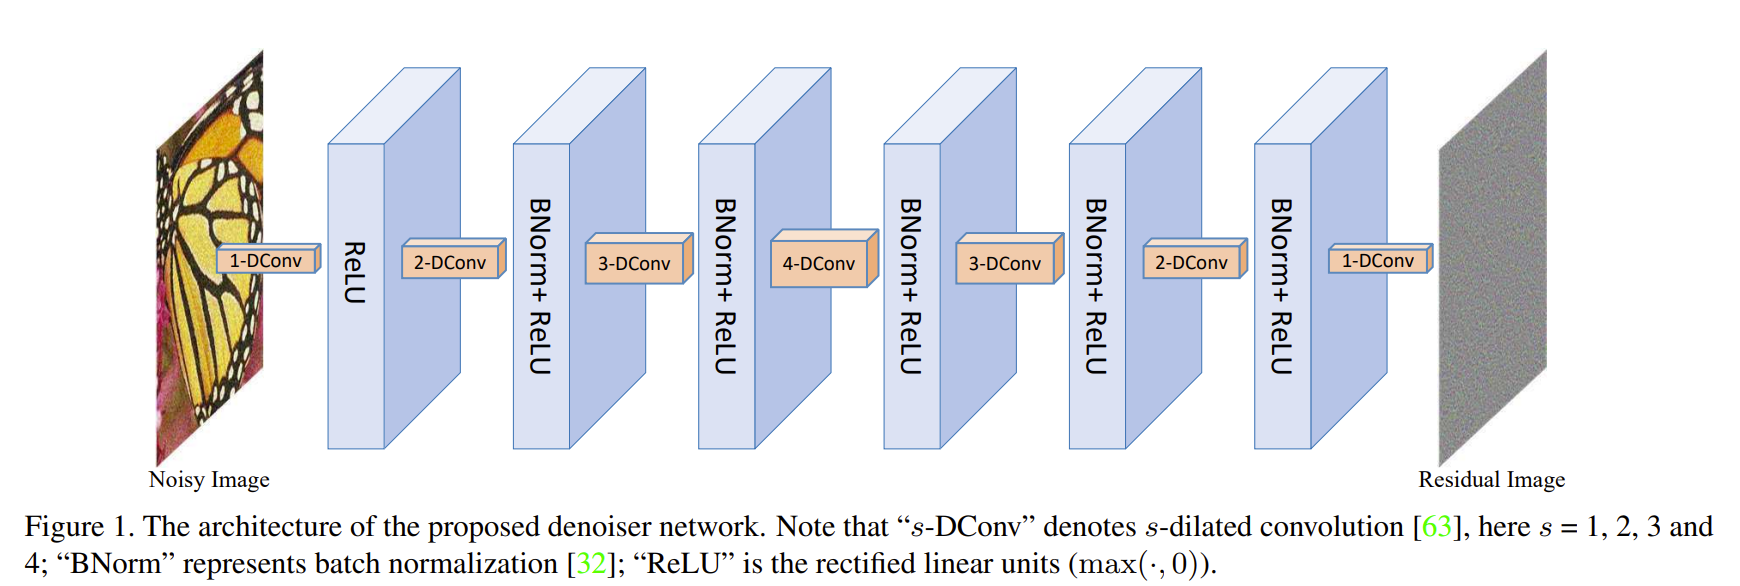
\includegraphics[width=\textwidth]{../paper/model.png}
        \caption{Denoiser utilisé dans l'article}
    \end{figure}
    \begin{block}{Méthodologie de l'article}
        Entraînement de 25 Denoiser avec une variance de bruit constant de $2k$ où $k\in [1, 25]$.
    \end{block}
\end{frame}

\begin{frame}{Denoiser: architecture}
    \begin{block}{Mon Denoiser}
        modèle : 5 couches CNNs au lieu de 7. (dilatation de 1, 2, 3, 2, 1) sur des images en 
        couleur de taille : $64 \times 64$.

        2 entraînements : 
        \begin{itemize}
            \item \textbf{Const}: a appris sur une variance de bruit constant de 5,
            les images viennent d'un maxpooling d'image de $256 \times 256$. \\

            \item \textbf{Rand}: a appris sur une variance de bruit uniforme sur $[1, 20]$, 
            les images qui viennent d'un crop.
        \end{itemize}
    \end{block}
\end{frame}

\begin{frame}{Le Denoiser: les résultats de tests}

    Les résultats de tests :
    \begin{table}
        \centering
        \begin{tabular}{|c|c|c|c|}
            \hline
             & MSE & PSNR & MSSSIM \\
             \hline
            \textbf{Baseline} & 3.74$\times 10^{-4}$ & 34.3 & 0.998\\
            \textbf{Const} & 7.05$\times 10^{-4}$ & 31.7 & 0.999 \\
            \hline
        \end{tabular}
        \caption{Image avec une variance de bruit constant de 5.}
    \end{table}

    \begin{table}
        \centering
        \begin{tabular}{|c|c|c|c|}
            \hline
             & MSE & PSNR & MSSSIM \\
             \hline
            \textbf{Baseline} & 18.7$\times 10^{-4}$ & 27.38 & 0.990\\
            \textbf{Rand} & 9.01$\times 10^{-4}$ & 30.6 & 0.996 \\
            \hline
        \end{tabular}
        \caption{Image avec une variance de bruit variant entre 1 et 20.}
    \end{table}
\end{frame}

\begin{frame}{Le Denoiser: inférence}
    Inférence du modèle : \textbf{Const}
    \begin{figure}[b]
        \centering
        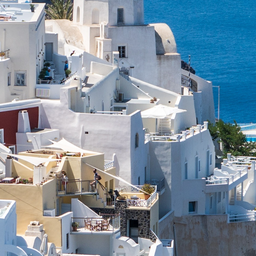
\includegraphics[width=0.30\textwidth]{../images/original/0823.png}
        
\includegraphics[width=0.30\textwidth]{../images/constant_blured/0823.png}
        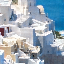
\includegraphics[width=0.30\textwidth]{../images/constant_infer/0823.png}
        \caption{image d'origine (à gauche), image bruitée (au centre) et image débruitée (à droite).}
    \end{figure}
\end{frame}

\begin{frame}{Le Denoiser: inférence}
    Inférence du modèle : \textbf{Rand}
    \begin{figure}[b]
        \centering
        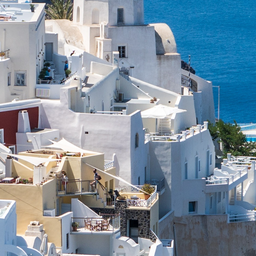
\includegraphics[width=0.30\textwidth]{../images/original/0823.png}
        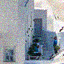
\includegraphics[width=0.30\textwidth]{../images/random_blured/0823.png}
        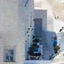
\includegraphics[width=0.30\textwidth]{../images/random_infer/0823.png}
        \caption{image d'origine (à gauche), image bruitée (au centre) et image débruitée (à droite).}
    \end{figure}
\end{frame}

% \section{implémentation}
\begin{frame}{Plug and play: résultats de \textbf{Const}}
    \begin{figure}[b]
        \centering
        
\includegraphics[width=0.20\textwidth]{../images/hqs_original/0823.png}
        \begin{tikzpicture}[overlay, remember picture]
            \draw[->, blue, very thick] (0,1.5) -- (1,1.5) node[midway, above, blue] {$f_{H, \sigma}$};
        \end{tikzpicture}
        \hspace{1cm}
        
\includegraphics[width=0.20\textwidth]{../images/hqs_constant/y.png}
        \caption{image d'origine x (à gauche) et l'image dégradée y (à droite).}
    \end{figure}
    \begin{figure}[b]
        \centering
        
\includegraphics[width=0.20\textwidth]{../images/hqs_constant/x_0.png}
        
\includegraphics[width=0.20\textwidth]{../images/hqs_constant/z_0.png}
        
\includegraphics[width=0.20\textwidth]{../images/hqs_constant/x_1.png}
        
\includegraphics[width=0.20\textwidth]{../images/hqs_constant/z_1.png}
        \caption{images représentant réspectivement $x_1$, $z_1$, $x_2$, $z_2$.}
    \end{figure}
\end{frame}

\begin{frame}{Plug and play : résultats de \textbf{Const}}
    Plug and play fait sur 10 itérations
    \begin{figure}[b]
        \centering
        
\includegraphics[width=0.30\textwidth]{../images/hqs_original/0823.png}
        
\includegraphics[width=0.30\textwidth]{../images/hqs_constant/y.png}
        
\includegraphics[width=0.30\textwidth]{../images/hqs_constant/z_9.png}
        \caption{image d'origine x non bruitée (à gauche), l'image dégradée y (au centre) et image de $z_{10}$ (à droite).}
    \end{figure}
\end{frame}

\begin{frame}{Plug and play : résultats de \textbf{Const}}
    \begin{figure}[b]
        \centering
        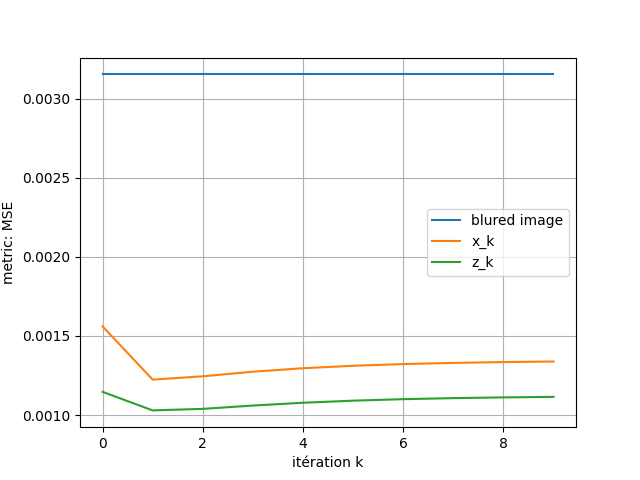
\includegraphics[width=0.49\textwidth]{../images/hqs_constant/MSE.png}
        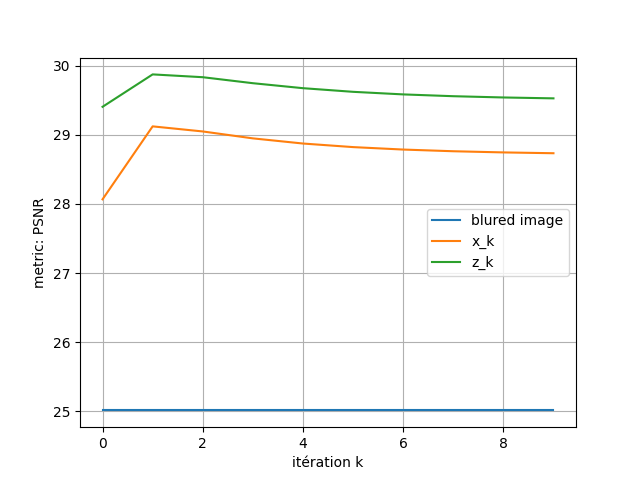
\includegraphics[width=0.49\textwidth]{../images/hqs_constant/PSNR.png}
        \caption{Métriques MSE et PSNR en fonction des itérations.}
    \end{figure}
\end{frame}

\begin{frame}{Plug and play : les résultats de l'article}
    Parler des résultats qu'ont obtenus les auteurs de l'article. (diapo pas encore faite)
\end{frame}

\begin{frame}{Plug and play : continue}
    Parler rapidement de la v2 du papier avec U-net (diapo pas encore faite)
\end{frame}

% \section{Références}
\begin{frame}{Références}
    \begin{itemize}
        \item \textbf{article:} Kai Zhang, Wangmeng Zuo, Shuhang Gu and Lei Zhang, 
            \textit{Learning Deep {CNN} Denoiser Prior for Image Restoration}.
            \url{http://arxiv.org/abs/1704.03264}
        \item \textbf{FISTA:} Amir Beck and Marc Teboulle, \textit{A Fast Iterative Shrinkage-Thresholding 
        Algorithm for Linear Inverse Problems}. \url{https://www.ceremade.dauphine.fr/~carlier/FISTA}
        \item \textbf{article v2:} Zhang, Kai and Li, Yawei and Zuo, Wangmeng and Zhang, Lei and Van Gool, Luc and Timofte, Radu,
            \textit{Plug-and-Play Image Restoration With Deep Denoiser Prior}, \url{https://arxiv.org/pdf/2008.13751.pdf}
        \item \textbf{Lien de mon implémentation :} \url{https://github.com/Highdrien/CNN-Denoiser-Prior}
    \end{itemize}
    
\end{frame}


\end{document}

